\begin{abox}
	Classical Mechanics
	\end{abox}
\begin{enumerate}
	\item Let $q$ and $p$ be the canonical coordinate and momentum of a dynamical system. Which of the following transformations is canonical?
	1. $Q_{1}=\frac{1}{\sqrt{2}} q^{2}$ and $P_{1}=\frac{1}{\sqrt{2}} p^{2}$
	2. $Q_{2}=\frac{1}{\sqrt{2}}(p+q)$ and $P_{2}=\frac{1}{\sqrt{2}}(p-q)$
{\exyear{ 	NET/JRF (June-2015)}}
	 \begin{tasks}(2)
		\task[\textbf{a.}] Neither 1 nor 2
		\task[\textbf{b.}]Both 1 and 2
		\task[\textbf{c.}] Only 1
		\task[\textbf{d.}] Only 2
	\end{tasks}
\begin{answer}
	$$
	\begin{aligned}
	\text { For } A: Q_{1}&=\frac{q^{2}}{\sqrt{2}}, P_{1}=\frac{P^{2}}{\sqrt{2}}\\
	\left[Q_{1}, P_{1}\right]&=\frac{\partial Q_{1}}{\partial q} \cdot \frac{\partial P_{1}}{\partial p}-\frac{\partial Q_{1}}{\partial p} \cdot \frac{\partial P_{1}}{\partial q} \neq 1\qquad \text{(Not canonical)}\\
	\text { For } B: Q_{2}&=\frac{1}{\sqrt{2}}(p+q), P_{2}=\frac{1}{\sqrt{2}}(p-q)\\
	\left[Q_{2}, P_{2}\right]&=1\qquad
	\text{(canonical)}
\end{aligned}
$$
So the correct answer is \textbf{Option(d)}
\end{answer}
	\item A canonical transformation relates the old coordinates $(q, p)$ to the new ones $(Q, P)$ by the relations $Q=q^{2}$ and $P=p / 2 q$. The corresponding time independent generating function is
{\exyear{ 	NET/JRF (June-2014)}}
	 \begin{tasks}(4)
		\task[\textbf{a.}]$P / q^{2}$
		\task[\textbf{b.}] $q^{2} P$
		\task[\textbf{c.}]$q^{2} / P$
		\task[\textbf{d.}] $q P^{2}$ 
	\end{tasks}
\begin{answer}
	$$
	\begin{aligned}
	Q&=q^{2} ; P=p / 2 q\\
	\frac{\partial F_{2}}{\partial q}&=p \Rightarrow \frac{\partial F_{2}}{\partial q}=P \cdot 2 q \Rightarrow F_{2}=q^{2} P+f(P)\\
	\frac{\partial F_{2}}{\partial P}&=Q=q^{2} \Rightarrow F_{2}=q^{2} P+f(q)\\
	\text { comparing both side } f(q)&=f(P)=0 \Rightarrow F_{2}=q^{2} P
\end{aligned}
$$
So the correct answer is \textbf{Option(b)}
\end{answer}
	\item A mechanical system is described by the Hamiltonian $H(q, p)=\frac{p^{2}}{2 m}+\frac{1}{2} m \omega^{2} q^{2}$. As a result of the canonical transformation generated by $F(q, Q)=-\frac{Q}{q}$, the Hamiltonian in the new coordinate $Q$ and momentum $P$ becomes
{\exyear{	NET/JRF (DEC-2014)}}
	 \begin{tasks}(2)
		\task[\textbf{a.}]$\frac{1}{2 m} Q^{2} P^{2}+\frac{m \omega^{2}}{2} Q^{2}$
		\task[\textbf{b.}]$\frac{1}{2 m} Q^{2} P^{2}+\frac{m \omega^{2}}{2} P^{2}$
		\task[\textbf{c.}]$\frac{1}{2 m} P^{2}+\frac{m \omega^{2}}{2} Q^{2}$
		\task[\textbf{d.}] $\frac{1}{2 m} Q^{2} P^{4}+\frac{m \omega^{2}}{2} P^{-2}$
	\end{tasks}
\begin{answer}
	$$
	\begin{aligned}
	H&=\frac{p^{2}}{2 m}+\frac{1}{2} m \omega^{2} q^{2}, \quad F=F_{1}(q, Q)=-\frac{Q}{q}\\
	\Rightarrow \frac{\partial F_{1}}{\partial q}&=p \Rightarrow \frac{Q}{q^{2}}=p\\
	\Rightarrow \frac{\partial F_{1}}{\partial Q}&=-P \Rightarrow-\frac{1}{q}=-P \Rightarrow q=\frac{1}{P}\\
	\text{From equation }&\text{(i) and (ii) }\Rightarrow p=Q P^{2}\qquad
	\because q=\frac{1}{P}\\
	H&=\frac{p^{2}}{2 m}+\frac{1}{2} m \omega^{2} q^{2}=\frac{Q^{2} P^{4}}{2 m}+\frac{1}{2} m \omega^{2}\left(\frac{1}{P^{2}}\right)=\frac{1}{2 m} Q^{2} P^{4}+\frac{1}{2} m \omega^{2} P^{-2}
\end{aligned}
$$
So the correct answer is \textbf{Option(d)}
\end{answer}
	\question Which of the following set of phase-space trajectories is not possible for a particle obeying Hamilton's equations of motion?
{\exyear{NET/JRF(DEC-2012)}}
\begin{tasks}(2)
\task[\textbf{A.}] \begin{figure}[H]
	\centering
	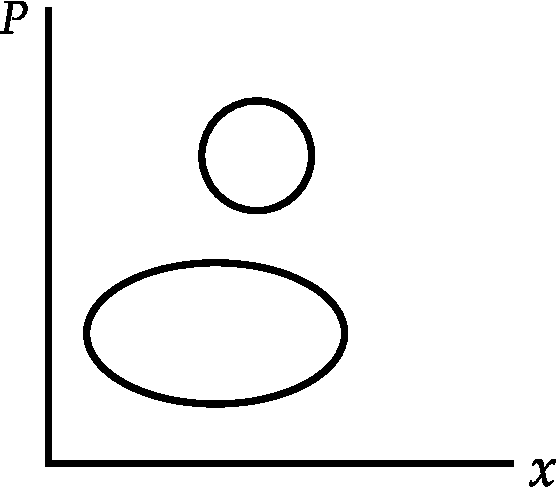
\includegraphics[height=4.5cm,width=5cm]{CMC-1}
\end{figure}
\task[\textbf{B.}] \begin{figure}[H]
	\centering
	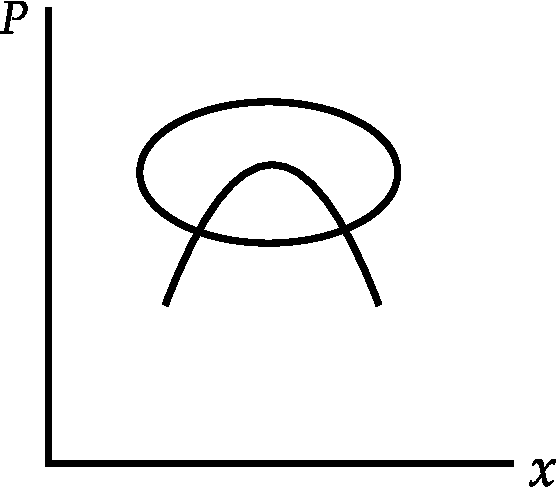
\includegraphics[height=4.5cm,width=5cm]{CMC-2}
\end{figure}
\task[\textbf{C.}] \begin{figure}[H]
	\centering
	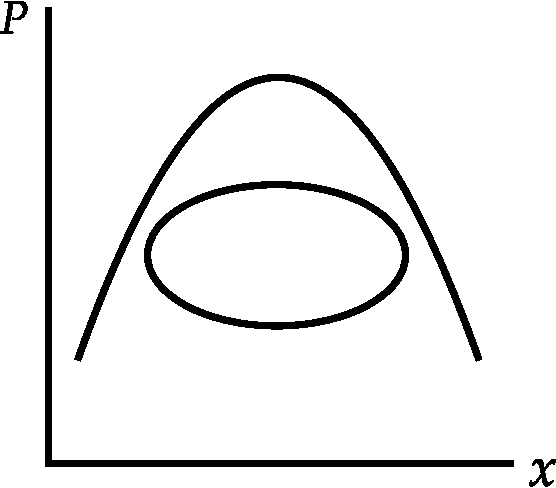
\includegraphics[height=4.5cm,width=5cm]{CMC-3}
\end{figure}
\task[\textbf{D.}] \begin{figure}[H]
	\centering
	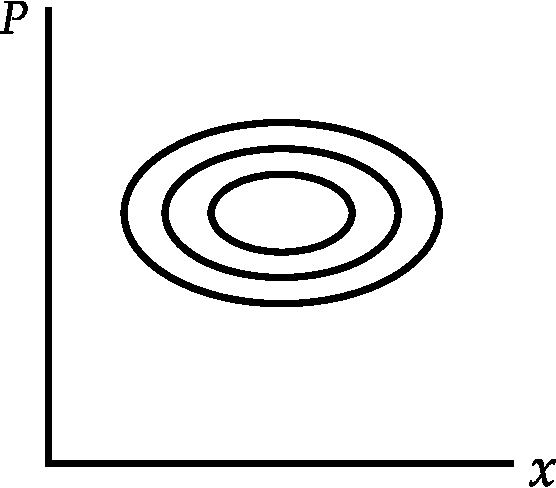
\includegraphics[height=4.5cm,width=5cm]{CMC-4}
\end{figure}
\end{tasks}
\begin{answer}
Phase curve does not cut each other\\\\
So the correct answer is \textbf{Option (B)}
\end{answer}
\item The trajectory on the $z p_{z}$ - plane (phase-space trajectory) of a ball bouncing perfectly elastically off a hard surface at $z=0$ is given by approximately by (neglect {friction):
	\exyear{NET/JRF(DEC-2011)}}
\begin{tasks}(2)
\task[\textbf{A.}] \begin{figure}[H]
	\centering
	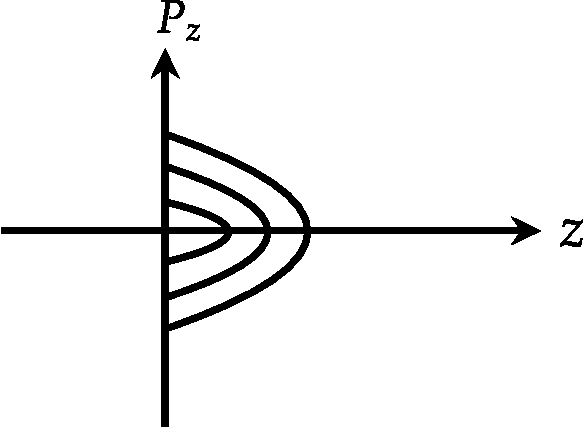
\includegraphics[height=4.5cm,width=5cm]{CMC-5}
\end{figure}
\task[\textbf{B.}] \begin{figure}[H]
	\centering
	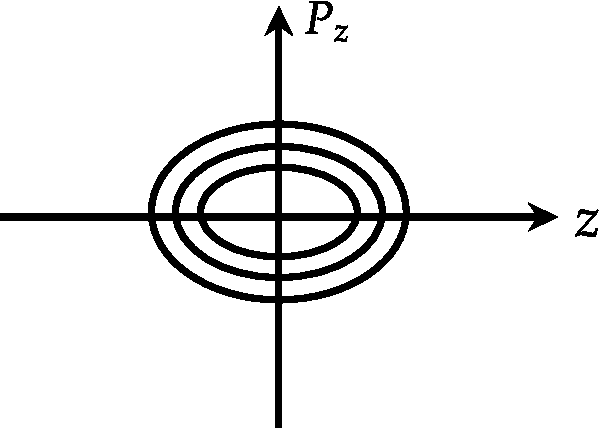
\includegraphics[height=4.5cm,width=5cm]{CMC-6}
\end{figure}
\task[\textbf{C.}] \begin{figure}[H]
	\centering
	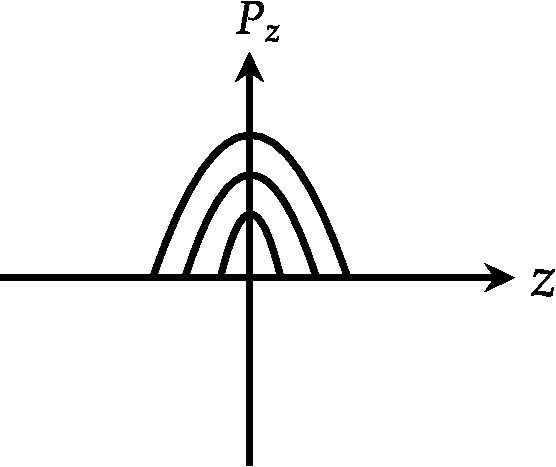
\includegraphics[height=4.5cm,width=5cm]{CMC-7}
\end{figure}
\task[\textbf{D.}] \begin{figure}[H]
	\centering
	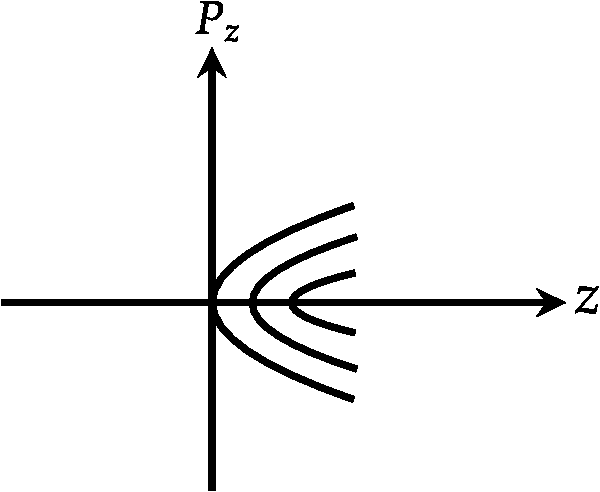
\includegraphics[height=4.5cm,width=5cm]{CMC-8}
\end{figure}
\end{tasks}
\begin{answer}
\begin{align*}
H=\frac{P_{z}^{2}}{2 m}+m g\text{ z and }E=\frac{P_{z}^{2}}{2 m}+m g z
\end{align*}
So the correct answer is \textbf{Option (A)}	
\end{answer}
\item The bob of a simple pendulum, which undergoes small oscillations, is immersed in water. Which of the following figures best represents the phase space diagram for the pendulum?
{\exyear{NET/JRF(JUNE-2012)}}
\begin{tasks}(2)
\task[\textbf{A.}] \begin{figure}[H]
	\centering
	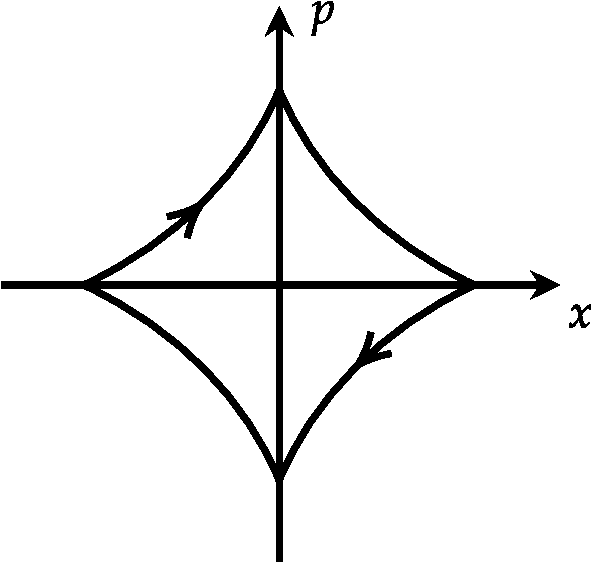
\includegraphics[height=4.5cm,width=5cm]{CMC-9}
\end{figure}
\task[\textbf{B.}] \begin{figure}[H]
	\centering
	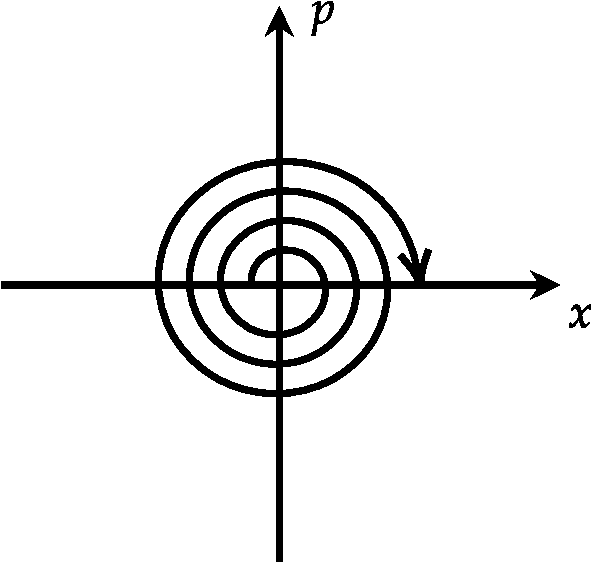
\includegraphics[height=4.5cm,width=5cm]{CMC-10}
\end{figure}
\task[\textbf{C.}] \begin{figure}[H]
	\centering
	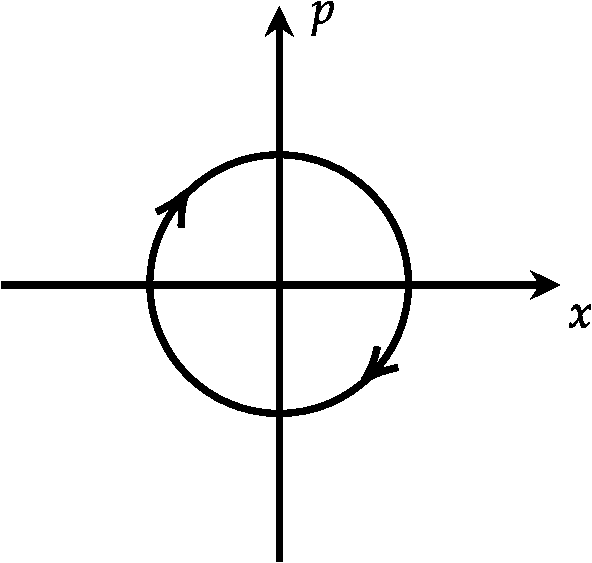
\includegraphics[height=4.5cm,width=5cm]{CMC-11}
\end{figure}
\task[\textbf{D.}] \begin{figure}[H]
	\centering
	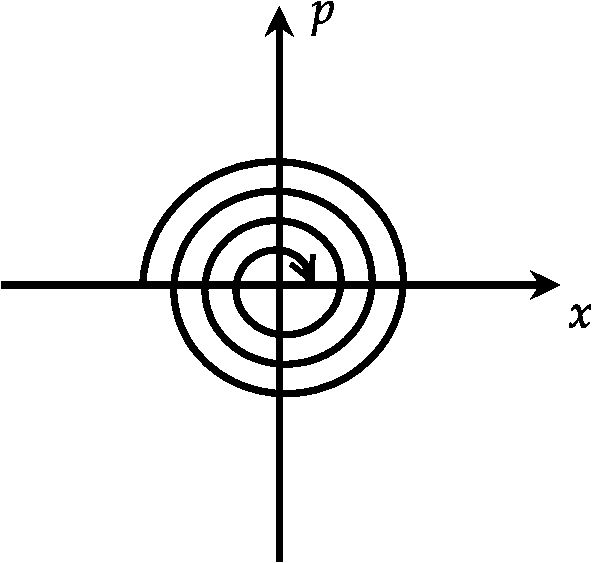
\includegraphics[height=4.5cm,width=5cm]{CMC-15}
\end{figure}
\end{tasks}
\begin{answer}
\begin{align*}
\intertext{When simple pendulum oscillates in water it is damped oscillation so amplitude continuously decrease and finally it stops.}
\end{align*}
So the correct answer is \textbf{Option (D)}
\end{answer}
\item Which of the following figures is a schematic representation of the phase space trajectories (i.e., contours of constant energy) of a particle moving in a one-dimensional potential $V(x)=\frac{-1}{2} x^{2}+\frac{1}{4} x^{4}$
{\exyear{NET/JRF(JUNE-2015)}}
\begin{tasks}(2)
\task[\textbf{A.}] \begin{figure}[H]
	\centering
	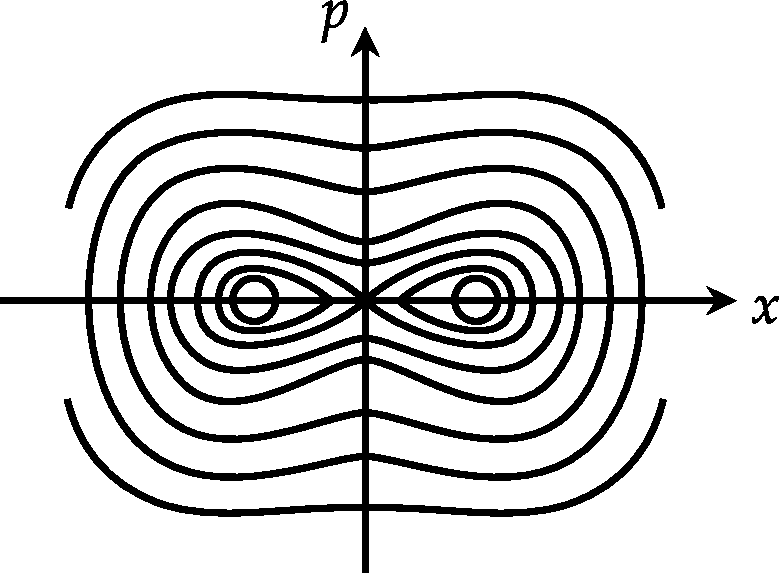
\includegraphics[height=4cm,width=5.5cm]{CMC-13}
\end{figure}
\task[\textbf{B.}] \begin{figure}[H]
	\centering
	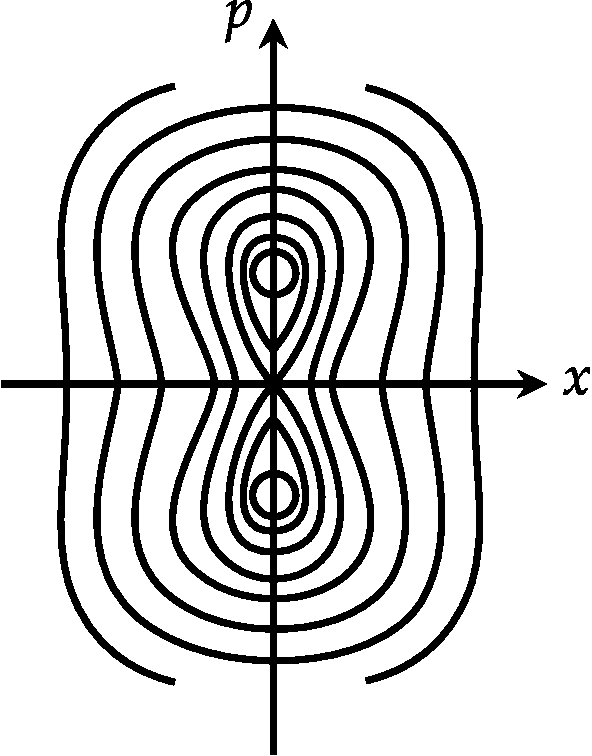
\includegraphics[height=5.5cm,width=4cm]{CMC-14}
\end{figure}
\task[\textbf{C.}] \begin{figure}[H]
	\centering
	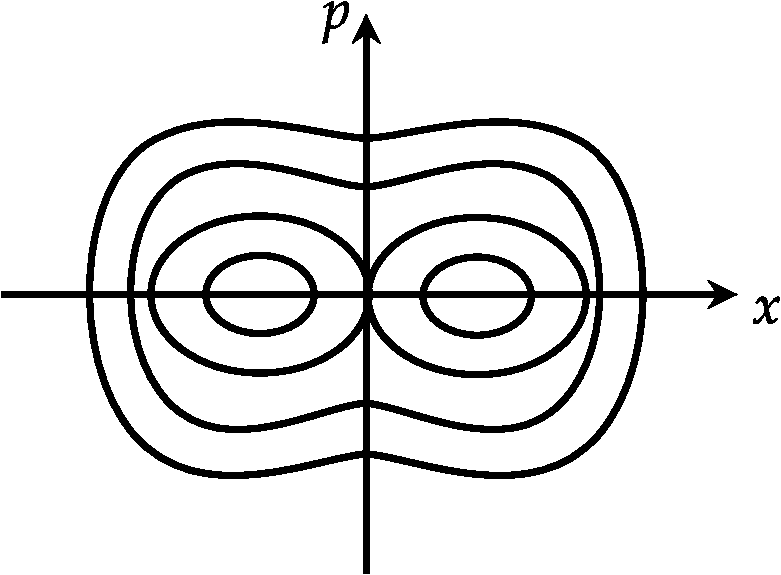
\includegraphics[height=4cm,width=5.5cm]{CMC-16}
\end{figure}
\task[\textbf{D.}] \begin{figure}[H]
	\centering
	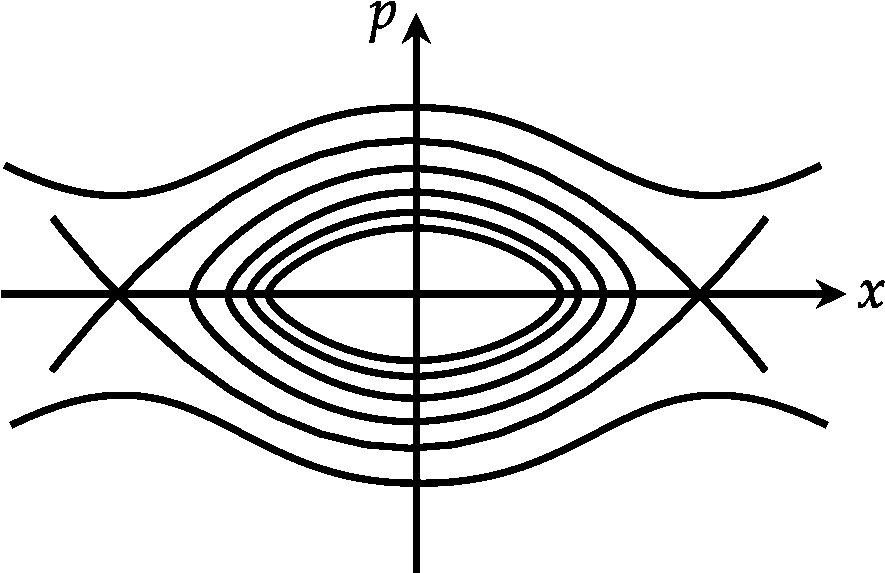
\includegraphics[height=4cm,width=5.5cm]{CMC-17}
\end{figure}
\end{tasks}
\begin{answer}$\left. \right. $
\begin{figure}[H]
	\centering
	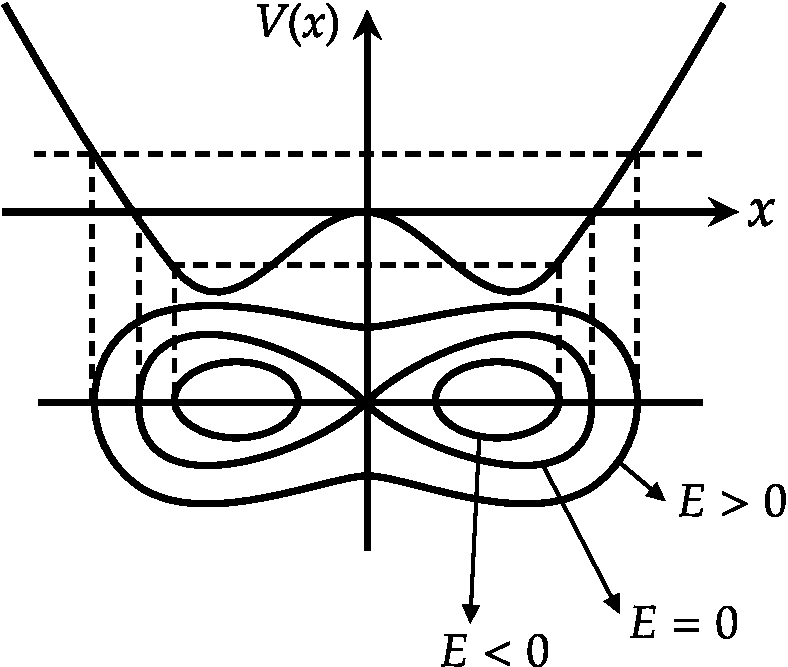
\includegraphics[height=5cm,width=6cm]{CMC-18}
\end{figure}
\begin{align*}
V(x)&=\frac{-x^{2}}{2}+\frac{x^{4}}{4}\\
\frac{\partial V}{\partial x}&=0 \Rightarrow x=0, x=\pm 1\\
\frac{\partial^{2} V}{\partial x^{2}}&=-v e\text{ for }x=0\text{ (unstable point)}\\
&=+\text{ ve for }x=\pm 1\text{ (stable point)}
\end{align*}
So the correct answer is \textbf{Option (A)}
\end{answer}
\item A particle of unit mass moves in a potential $V(x)=a x^{2}+\frac{b}{x^{2}}$, where $a$ and $b$ are positive constants. The angular frequency of small oscillations about the minimum of the potential is
{\exyear{NET/JRF(JUNE-2011)}}
\begin{tasks}(4)
\task[\textbf{A.}] $\sqrt{8 b}$
\task[\textbf{B.}] $\sqrt{8 a}$
\task[\textbf{C.}] $\sqrt{8 a / b}$
\task[\textbf{D.}] $\sqrt{8 b / a}$
\end{tasks}
\begin{answer}
\begin{align*}
V(x)&=a x^{2}+\frac{b}{x^{2}} \Rightarrow \frac{\partial V}{\partial x}=0 \Rightarrow 2 a x-\frac{2 b}{x^{3}}\\&=0 \Rightarrow a x^{4}-b=0 \Rightarrow x_{0}=\left(\frac{b}{a}\right)^{\frac{1}{4}}\\
\text{Since }\omega&=\sqrt{\frac{k}{m}}, m=1\text{ and }k=\left.\frac{\partial^{2} V}{\partial x^{2}}\right|_{x=x_{0}}\text{ where }x_{0} \text{ is stable equilibrium point,}\\
\text{Hence }k&=\frac{\partial^{2} V}{\partial x^{2}}=2 a+\frac{6 b}{x_{0}^{4}}\\&=2 a+\frac{6 b}{b / a}=8 a\text{ at }x=x_{0}=\left(\frac{b}{a}\right)^{\frac{1}{4}}\\
\text{Thus, }\omega&=\sqrt{8 a}
\end{align*}
So the correct answer is \textbf{Option (B)}
\end{answer}
\item The potential of a diatomic molecule as a function of the distance $r$ between the atoms is given by $V(r)=-\frac{a}{r^{6}}+\frac{b}{r^{12}} .$ The value of the potential at equilibrium separation between the atoms is:
{\exyear{NET/JRF(DEC-2011)}}
\begin{tasks}(4)
\task[\textbf{A.}] $-4 a^{2} / b$
\task[\textbf{B.}] $-2 a^{2} / b$
\task[\textbf{C.}] $-a^{2} / 2 b$
\task[\textbf{D.}] $-a^{2} / 4 b$
\end{tasks}
\begin{answer}
\begin{align*}
V(r&=-\frac{a}{r^{6}}+\frac{b}{r^{12}},\text{ for equilibrium }\frac{\partial V}{\partial r}\\&=0 \Rightarrow-(-6) \frac{\mathrm{a}}{\mathrm{r}^{7}}-\frac{12 \mathrm{~b}}{\mathrm{r}^{13}}\\&=0 \Rightarrow \frac{1}{r^{7}}\left[6 a-\frac{12 b}{r^{6}}\right]=0\\
\Rightarrow 6 a-\frac{12 b}{r^{6}}&=0 \Rightarrow r=\left(\frac{12 b}{6 a}\right)^{\frac{1}{6}} \Rightarrow r=\left(\frac{2 b}{a}\right)^{\frac{1}{6}}\\
\Rightarrow V\left(r=\left(\frac{2 b}{a}\right)^{\frac{1}{6}}\right)&=-\frac{a}{\left(\frac{2 b}{a}\right)}+\frac{b}{\left(\frac{2 b}{a}\right)^{2}}\\&=-\frac{a^{2}}{2 b}+\frac{a^{2}}{4 b}=-\frac{a^{2}}{4 b}
\end{align*}
So the correct answer is \textbf{Option (D)}
\end{answer}
\item Consider the motion of a classical particle in a one dimensional double-well potential $V(x)=\frac{1}{4}\left(x^{2}-2\right)^{2}$. If the particle is displaced infinitesimally from the minimum on the $x$-axis (and friction is neglected), then
{\exyear{NET/JRF(JUNE-2012)}}
\begin{tasks}(1)
\task[\textbf{A.}] The particle will execute simple harmonic motion in the right well with an angular frequency $\omega=\sqrt{2}$
\task[\textbf{B.}] The particle will execute simple harmonic motion in the right well with an angular frequency $\omega=2$
\task[\textbf{C.}] The particle will switch between the right and left wells
\task[\textbf{D.}]  The particle will approach the bottom of the right well and settle there
\end{tasks}
\begin{answer}
\begin{align*}
V(x)&=\frac{1}{4}\left(x^{2}-2\right)^{2} \Rightarrow \frac{\partial V}{\partial x}\\&=\frac{2}{4}\left(x^{2}-2\right) \times 2 x=0 \Rightarrow x=0, x=\pm \sqrt{2}
\intertext{$\frac{\partial^{2} V}{\partial x^{2}}=3 x^{2}-2$. At $x=0, \frac{\partial^{2} V}{\partial x^{2}}<0$ so $V$ is maximum. Thus it is unstable point $\left.\frac{\partial^{2} V}{\partial x^{2}}\right|_{x=\pm \sqrt{2}}=4$ and it is stable equilibrium point with $\omega=\sqrt{\frac{\left.\frac{\partial^{2} V}{\partial x^{2}}\right|_{x=x_{0}}}{\mu}}=2 \quad \because \mu=1$}
\end{align*}
So the correct answer is \textbf{Option (B)}
\end{answer}
\item A solid cylinder of height $H$, radius $R$ and density $\rho$, floats vertically on the surface of a liquid of density $\rho_{0} .$ The cylinder will be set into oscillatory motion when a small instantaneous downward force is applied. The frequency of oscillation is
{\exyear{NET/JRF(DEC-2012)}}
\begin{tasks}(4)
\task[\textbf{A.}] $\frac{\rho g}{\rho_{0} H}$
\task[\textbf{B.}]  $\frac{\rho}{\rho_{0}} \sqrt{\frac{g}{H}}$
\task[\textbf{C.}] $\sqrt{\frac{\rho g}{\rho_{0} H}}$
\task[\textbf{D.}] $\sqrt{\frac{\rho_{0} g}{\rho H}}$
\end{tasks}
\begin{answer}
\begin{align*}
\intertext{Solution: From Newton's law of motion $m a=m g-\rho_{0} A g h$ where $A$ is area of cross section, $m=\rho A H$}
\Rightarrow \rho A H a&=\rho A H g-\rho_{0} A g h \Rightarrow a=1-\frac{\rho_{0} g h}{\rho H} \Rightarrow \omega=\sqrt{\frac{\rho_{0} g}{\rho H}}
\end{align*}
So the correct answer is \textbf{Option (D)}
\end{answer}
\item A solid vertical rod, of length $L$ and cross-sectional area $A$, is made of a material of Young's modulus $Y$. The rod is loaded with a mass $M$, and, as a result, extends by a small amount $\Delta L$ in the equilibrium condition. The mass is then suddenly reduced to $M / 2$. As a result the rod will undergo longitudinal oscillation with an angular frequency
{\exyear{NET/JRF(JUNE-2017)}}
\begin{tasks}(4)
\task[\textbf{A.}] $\sqrt{2 Y A / M L}$
\task[\textbf{B.}] $\sqrt{Y A / M L}$
\task[\textbf{C.}] $\sqrt{2 Y A / M \Delta L}$
\task[\textbf{D.}] $\sqrt{Y A / M \Delta L}$
\end{tasks}
\begin{answer}
\begin{align*}
Y&=\frac{F l}{A \Delta l} \Rightarrow F=\frac{Y A \Delta l}{l}\\
\text{For mass }m, \quad m g&=\frac{Y A \Delta l}{l}\\
\text{For mass }\frac{m}{2} g&=\frac{Y A}{l}\left(\frac{\Delta l}{2}\right)
\intertext{Equation (i) and (ii) is for equilibrium condition}
\intertext{Change in force will generate acceleration}
\Delta F&=\left(\frac{m g}{2}-m g\right)=\frac{Y A}{l}\left(\frac{\Delta l}{2}-\Delta l\right)=\frac{Y A}{2} \frac{\Delta l}{l}\\
\frac{-m \omega^{2} \Delta l}{2}&=\frac{Y A}{l} \frac{\Delta l}{2}\\
\omega&=\sqrt{\frac{Y A}{m l}}
\end{align*}
So the correct answer is \textbf{Option (B)}
\end{answer}
\item The time period of a simple pendulum under the influence of the acceleration due to gravity $g$ is $T$. The bob is subjected to an additional acceleration of magnitude $\sqrt{3} g$ in the horizontal direction. Assuming small oscillations, the mean position and time period of oscillation, respectively, of the bob will be
{\exyear{NET/JRF(JUNE-2014)}}
\begin{tasks}(2)
\task[\textbf{A.}]  $0^{\circ}$ to the vertical and $\sqrt{3} T$
\task[\textbf{B.}] $30^{\circ}$ to the vertical and $T / 2$
\task[\textbf{C.}] $60^{\circ}$ to the vertical and $T / \sqrt{2}$
\task[\textbf{D.}] $0^{\circ}$ to the vertical and $T / \sqrt{3}$
\end{tasks}
\begin{answer}
\begin{figure}[H]
	\centering
	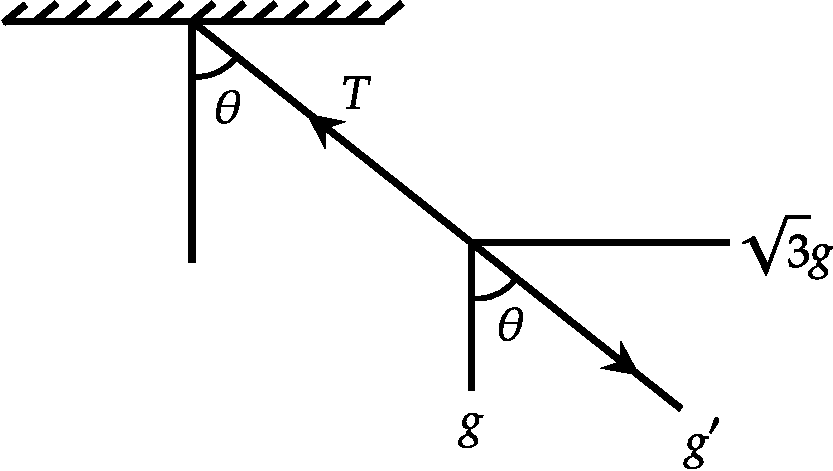
\includegraphics[height=4.5cm,width=7cm]{CMC-19}
\end{figure}
\begin{align*}
T&=2 \pi \sqrt{\frac{l}{g}}\\
g^{\prime}&=\sqrt{3 g^{2}+g^{2}}=\sqrt{4 g^{2}}=2 g\\
T^{\prime}&=2 \pi \sqrt{\frac{l}{2 g}} \Rightarrow T^{\prime}\\&=2 \pi \sqrt{\frac{l}{g}} \cdot \frac{1}{\sqrt{2}} \Rightarrow T^{\prime}=\frac{T}{\sqrt{2}}\\
T \cos \theta&=m g, T \sin \theta=\sqrt{3} m g \Rightarrow \tan \theta\\&=\sqrt{3} \Rightarrow \theta=60^{\circ}
\end{align*}
So the correct answer is \textbf{Option (C)}
\end{answer}
\item Three particles of equal mass $(\mathrm{m})$ are connected by two identical massless springs of stiffness constant $(\mathrm{K})$ as shown in the figure\\
\begin{figure}[H]
	\centering
	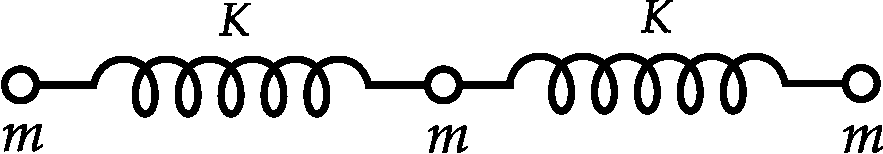
\includegraphics[height=1.3cm,width=7cm]{CMC-20}
\end{figure}
If $x_{1}, x_{2}$ and $x_{3}$ denote the horizontal displacement of the masses from their respective equilibrium positions the potential energy of the system is
{\exyear{NET/JRF(DEC-2012)}}
\begin{tasks}(2)
\task[\textbf{A.}] $\frac{1}{2} K\left[x_{1}^{2}+x_{2}^{2}+x_{3}^{2}\right]$
\task[\textbf{B.}] $\frac{1}{2} K\left[x_{1}^{2}+x_{2}^{2}+x_{3}^{2}-x_{2}\left(x_{1}+x_{3}\right)\right]$
\task[\textbf{C.}] $\frac{1}{2} K\left[x_{1}^{2}+2 x_{2}^{2}+x_{3}^{2}-2 x_{2}\left(x_{1}+x_{3}\right)\right]$
\task[\textbf{D.}] $\frac{1}{2} K\left[x_{1}^{2}+2 x_{2}^{2}-2 x_{2}\left(x_{1}+x_{3}\right)\right]$
\end{tasks}
\begin{answer}
\begin{align*}
V&=\frac{1}{2} K\left(x_{2}-x_{1}\right)^{2}+\frac{1}{2} K\left(x_{3}-x_{2}\right)^{2}\\
V&=\frac{1}{2} K\left(x_{2}^{2}+x_{1}^{2}-2 x_{2} x_{1}\right)+\frac{1}{2} K\left(x_{3}^{2}+x_{2}^{2}-2 x_{3} x_{2}\right) \Rightarrow V\\&=\frac{1}{2} K\left[x_{1}^{2}+2 x_{2}^{2}+x_{3}^{2}-2 x_{2}\left(x_{1}+x_{3}\right)\right]
\end{align*}
So the correct answer is \textbf{Option (C)}
\end{answer}
\item The Lagrangian of a system is given by
$$
L=\frac{1}{2} m \dot{q}_{1}^{2}+2 m \dot{q}_{2}^{2}-k\left(\frac{5}{4} q_{1}^{2}+2 q_{2}^{2}-2 q_{1} q_{2}\right)
$$
where $m$ and $k$ are positive constants. The frequencies of its normal modes are
{\exyear{NET/JRF(DEC-2015)}}
\begin{tasks}(2)
\task[\textbf{A.}] $\sqrt{\frac{k}{2 m}}, \sqrt{\frac{3 k}{m}}$
\task[\textbf{B.}] $\sqrt{\frac{k}{2 m}}(13 \pm \sqrt{73})$
\task[\textbf{C.}] $\sqrt{\frac{5 k}{2 m}}, \sqrt{\frac{k}{m}}$
\task[\textbf{D.}]  $\sqrt{\frac{k}{2 m}}, \sqrt{\frac{6 k}{m}}$
\end{tasks}
\begin{answer}
\begin{align*}
L&=\frac{1}{2} m \dot{q}_{1}^{2}+2 m \dot{q}_{2}^{2}-k\left[\frac{5}{4} q_{1}^{2}+2 q_{2}^{2}-2 q_{1} q_{2}\right]\\
L&=\frac{1}{2} m \dot{q}_{1}^{2}+\frac{4}{2} m \dot{q}_{2}^{2}-\frac{k}{2}\left[\frac{10}{4} q_{1}^{2}+4 q_{2}^{2}-2 q_{1} q_{2}-2 q_{2} q_{1}\right]\\
T&=\left(\begin{array}{cc}m & 0 \\ 0 & 4 m\end{array}\right), \quad V=\left(\begin{array}{cc}\frac{10}{4} k & -2 k \\ -2 k & 4 k\end{array}\right)
\intertext{The secular equation $\left|V-\omega^{2} m\right|=0$}
\left(\begin{array}{cc}\frac{10}{4} k-\omega^{2} m & -2 k \\ -2 k & 4 k-\omega^{2} 4 m\end{array}\right)&=0,\left(\frac{10}{4} k-\omega^{2} m\right)\left(4 k-4 \omega^{2} m\right)-4 k^{2}=0\\
&\Rightarrow 10 k^{2}-10 \omega^{2} k m-4 \omega^{2} k m+4 \omega^{4} m^{2}-4 k^{2}=0\\
&\Rightarrow 3 k^{2}-7 \omega^{2} k m+2 \omega^{4} m^{2}\\&=0 \Rightarrow 3 k^{2}-6 \omega^{2} k m-\omega^{2} k m+2 \omega^{4} m^{2}=0\\
&\Rightarrow\left(k-2 \omega^{2} m\right)\left(3 k-\omega^{2} m\right)=0 \Rightarrow \omega\\&=\sqrt{\frac{k}{2 m}}, \quad \omega=\sqrt{\frac{3 k}{m}}
\end{align*}
So the correct answer is \textbf{Option (A)}
\end{answer}
\end{enumerate}